\chapter{Mise en \oe uvre numérique de l'algorithme de propagation}
\label{chap:methode_numerique}

Dans ce chapitre, on propose une mise en \ou euvre numérique de l'algorithme présenté au chapitre précédent. 
\begin{enumerate}
	\item choix de la discrétisation spatiale
	\begin{itemize}
		\item représentation des carreaux de surface
		\item représentation (et calcul) des courbes d'intersection entre carreaux
	\end{itemize}
	\item intégration temporelle
	\begin{itemize}
		\item intégration explicite du champ de vitesse 
		\item construction géométrique discrète de l'EdB suivant une méthode pseudo-spectrale (exacte aux points de collocation + interpolation)
	\end{itemize}
	\item considérations sur la stabilité numérique
\end{enumerate}



%\section{Discrétisation (pseudo-)spectrale en espace}
\section{Représentation des carreaux de surface}
\subsection{État de l'art}
\begin{enumerate}
	\item harmoniques sphériques \cite{rahimian2015}
	\item polynômes trigonométriques \cite{gueyffier2015}
	\item[$\Rightarrow$] limitations géométriques (régularité globale) et topologique (périodicité)
	\item modèle \brep\ permet une plus grande flexibilité
	\item polynômes algébriques (en produit tensoriel) adaptés aux carreaux de surface
	\item CAO : Bezier, NURBS $\to$ base des polynômes de Bernstein
	\begin{itemize}
		\item $B_n^N(x) = \binom{N}{n} \left( 1 - x \right)^{N-n} x^n$ pour $0 \leq n \leq N$.
		\item positivité : pour $0 \leq x \leq 1$, $B_n^N(x) \geq 0$
		\item partition de l'unité : $\sum_{n = 0}^N B_n^N = 1$
		\item[$\to$] propriétés intéressantes pour la conception géométrique
		\begin{itemize}
			\item coefficients = points de contrôle
			\item l'enveloppe convexe des points de contrôle englobe la courbe/surface de Bézier
		\end{itemize}
		\item inconvénients :
		\begin{itemize}
			\item points de contrôle pas \emph{sur} la courbe/surface $\Rightarrow$ pas exploitables comme marqueurs lagrangiens
			\item algorithme d'évaluation (de Casteljau) numériquement stable mais coûteux $\bigO{N^2}$
		\end{itemize}
	\end{itemize}
	\item motivation le choix des polynômes de Chebyshev
\end{enumerate}

%\subsection{Polynômes de Bernstein}
%Les polynômes de Bernstein sont définis par
%\begin{equation}
%	B_n^N(x) = \binom{N}{n} \left( 1 - x \right)^{N-n} x^n,
%	\label{eq:bernstein_poly}
%\end{equation}
%pour $0 \leq n \leq N$.
%Propriétés :
%\begin{itemize}
%	\item positivité : pour $0 \leq x \leq 1$, $B_n^N(x) \geq 0$
%	\item partition de l'unité : $\sum_{n = 0}^N B_n^N = 1$
%	\item dérivée : ${B_n^N}' = N \left( B_{n-1}^{N-1} - B_n^{N-1} \right)$
%\end{itemize}
%Avantages/inconvénients
%\begin{itemize}
%	\item[$+$] coefficients = points de contrôle dans l'espace physique, sens géométrique intuitif
%	\item[$+$] partition de l'unité sur $\berninterval$ $\Rightarrow$ propriété d'enveloppe convexe
%	\item[$\pm$] algorithme d'évaluation (de Casteljau) numériquement stable mais coûteux $\bigO{N^2}$
%	\item[$-$] points de contrôle pas \emph{sur} la courbe/surface $\Rightarrow$ pas exploitables comme marqueurs lagrangiens
%	\item[$-$] peu pratiques pour réduire/élever le degré des polynômes
%\end{itemize}


\subsection{Polynômes de Chebyshev univariés}
Les polynômes de Chebyshev sont très largement utilisés dans de nombreux domaines tels que l'analyse numérique.
L'objet des sections suivantes est de rappeler la définition de cette famille de polynômes et d'en présenter brièvement les propriétés remarquables qui seront exploitées dans cette thèse. 
Nombreux sont les ouvrages consacrés aux polynômes de Chebyshev \cite{mason2002, gil2007} ainsi qu'à leur usage dans les méthodes spectrales \cite{boyd2001, canuto2006}, aussi le lecteur est invité à s'y référer pour plus de détails.

\subsubsection{Définition et principales propriétés}
\begin{definition}
	Pour $n \in \mathbb{N}$, le polynôme de Chebyshev (de première espèce) $T_n$ est défini par%un polynome de degré $n$ défini par
	\begin{equation}
		T_n(\cos \theta) = n \cos \theta.
		\label{eq:chebyshev_trigo}
	\end{equation}
\end{definition}
%De la définition \eqref{eq:chebyshev_trigo} et de l'identité trigonométrique
De cette définition et de l'identité trigonométrique $\cos n\theta + \cos (n-2)\theta = 2\cos \theta \cos (n-1)\theta$, on peut déduire la relation de récurrence suivante, pour $-1 \leq x \leq 1$, 
\begin{align}[left = \empheqlbrace\,]
	T_0(x) &= 1, \nonumber\\
	T_1(x) &= x, \nonumber\\
	T_n(x) &= 2x T_{n-1}(x) - T_{n-2}(x) \text{,\ pour\ } n \geq 2.
	\label{eq:chebyshev_recurrence}
\end{align}
Le graphe des six premiers polynômes de Chebyshev est tracé sur la \autoref{fig:chebyshev_polynomials}.\par

\begin{figure}
	\centering
	%https://tex.stackexchange.com/questions/127375/replicate-the-fourier-transform-time-frequency-domains-correspondence-illustrati
\begin{tikzpicture}[%
		ax/.style={on layer=background, black, line width=0.5pt},
		grid/.style={on layer=background, black!25, line width=0.4pt},
		tickl/.style={font=\small},
		myax/.style={}
	]%
	\begin{axis}[
	width=12cm, height=9cm,
    set layers=standard,
    %domain=-1:1,
    xmin=-1, xmax=1,
    zmin=-1, zmax=1,
    samples y=1,
    view={40}{30},
    %hide axis,
    axis line style={draw=none},
    tick style={draw=none},
    grid = none,
    axis lines* = left,
    unit vector ratio*=4 3 1,
    %xtick=\empty, ytick=\empty, ztick=\empty,
    xtick={-1,-0.5,0,0.5,1},
    ytick={0,1,2,3,4,5},
    ztick={-1,0,1},
    %xlabel={$x$},
    %ylabel={$n$},
    %zlabel={$T_n(x)$},
    yticklabels=\empty,
    %zticklabels=\empty,
    no marks,
    samples=201,
    every tick label/.append style={font=\small},
    %tick align=outside,
%    cycle list/GnBu-9,%RdYlBu-6,%Spectral-6,
%	cycle multiindex* list={GnBu-9},%RdYlBu-6}%Spectral-6}
    clip=false
]
% x,z grid lines (at y=cst)
\foreach \y in {0,1,...,5}{%
	\foreach \x in {{-0.5},{0},{0.5},{1}}{
		\begingroup\edef\temp{\endgroup\noexpand\draw [grid] (axis cs:\x,\y,-1) -- ++ (axis direction cs:0,0,2);}\temp
	}
	\foreach \z in {{0},{1}}{
		\begingroup\edef\temp{\endgroup\noexpand\draw [grid] (axis cs:-1,\y,\z) -- ++ (axis direction cs:2,0,0,0);}\temp
	}
}
\pgfplotsinvokeforeach{0,1,...,5}{%
	\addplot3+[domain=-1:1]	({x},#1,{ cos(#1*acos(x)) });
%	\node[font=\footnotesize, anchor=west, inner sep=0] 
%		at (axis cs:1,#1,-0.3) {$n = #1$};
	\draw [ax] (axis cs:-1,#1,-1) -- ++ (axis direction cs:2,0,0); % x-axis
	\draw [ax] (axis cs:-1,#1,-1) -- ++ (axis direction cs:0,0,2); % z-axis
}%
% x,z ticks
\foreach \y in {0,1,...,5}{%
	\foreach \x in {{-1},{-0.5},{0},{0.5},{1}}{
		\begingroup\edef\temp{\endgroup\noexpand\draw [ax] (axis cs:\x,\y,-1) -- ++ (axis direction cs:0,0,0.2);}\temp
	}
	\foreach \z in {{-1},{0},{1}}{
		\begingroup\edef\temp{\endgroup\noexpand\draw [ax] (axis cs:-1,\y,\z) -- ++ (axis direction cs:0.05,0,0,0);}\temp
	}
}
% x, z tick labels and grid lines
%\pgfplotsinvokeforeach{-1,-0.5,0,0.5,1}{
%	\node[anchor=north, myax, tickl, xshift=-4pt] at (axis cs:#1,0,-1.1) {$#1$};
%%	\draw [grid] (axis cs:#1,0,-1) -- ++ (axis direction cs:0,5,0);
%}
%\pgfplotsinvokeforeach{-1,0,1}{
%	\node[anchor=east, myax, tickl] at (axis cs:-1,0,#1) {$#1$};
%%	\draw [grid] (axis cs:-1,0,#1) -- ++ (axis direction cs:0,5,0);
%}
% x,z labels
\node[anchor=north west, myax] at (axis cs:0,-1.1,-1) {$x$};
\node[anchor=south, rotate=90, myax, inner sep=7mm] at (axis cs:-1,0,0) {$T_n(x)$};
%
% y axis
\draw[ax, -latex] (axis cs:1.25,0,-1) -- ++ (axis direction cs:0,5.5,0) node[anchor=south west] {$n$};
\pgfplotsinvokeforeach{0,1,...,5}{%
	\draw[ax] (axis cs:1.25,#1,-1) -- ++ (axis direction cs:-0.05,0,0);
	\node[anchor=north west, myax, tickl] at (axis cs:1.25,#1,-1) {$#1$};
}
%\foreach \n in {0,1,...,5}{%
%	\node[font=\footnotesize, anchor=west, inner sep=0] 
%		at (axis cs:1,\n,-0.3) {$n = \n$};
%	\draw [ax] (axis cs:-1,\n,-1) -- ++ (axis direction cs:2,0,0); % x-axis
%	\draw [ax] (axis cs:-1,\n,-1) -- ++ (axis direction cs:0,0,2); % z-axis
%	\foreach \z in {-1,0,1}{%
%		\draw [ax] (axis cs:-1,\n,\z) -- ++ (axis direction cs:0.025,0,0);
%	}%
%	\foreach \x in {-1,-0.5,0,0.5,1}{%
%		\draw [ax] (axis cs:\x,\n,-1) -- ++ (axis direction cs:0,0,0.1);
%	}%
%}%
\end{axis}
\end{tikzpicture}
	\caption{Graphe des six premiers polynômes de Chebyshev.}% $(n=0,\ldots,5)$ sur l'intervalle $\chebinterval$.}
	\label{fig:chebyshev_polynomials}
\end{figure}

$T_n$ est un polynôme de degré $n$ %de coefficient dominant $2^{n-1}$ 
qui atteint ses extrema locaux sur $\chebinterval$ aux $n+1$ n\oe uds de Chebyshev-Gauss-Lobatto (CGL)%\footnote{Seuls les $n-1$ n\oe uds intérieurs sont réellement des extrema au sens où la dérivée s'y annule. A noter également que ces n\oe uds sont rangés en ordre décroissant.}
\begin{equation}
	x_k = \cos \frac{k \pi}{n},
	\label{eq:cgl_nodes}
\end{equation}
pour $0 \leq k \leq n$. 
Seuls les $n-1$ n\oe uds intérieurs sont réellement des extrema au sens où la dérivée s'y annule. 
À noter également que ces n\oe uds sont rangés en ordre décroissant.\par

\begin{figure}
	\centering
	\begin{tikzpicture} 
	\begin{axis}[%
		width=8cm, height=6cm,
		axis lines*=left,
		xmin=-1.0, xmax=1.0, ymin=-1.0, ymax=1.0,
		grid=major,
		clip marker paths=false,
		enlargelimits={abs=0.05},
		]%
		\addplot+[samples=200, domain=0:pi, no marks, mycolor_6] ({cos(deg(x))}, {cos(5*deg(x))});%
		% extrema
		\addplot+[samples=6, domain=0:pi, ycomb, dashed, mark=none, black] ({cos(deg(x))}, {cos(5*deg(x))});%
		\addplot+[samples=6, domain=0:pi, only marks, mark=*, black] ({cos(deg(x))}, {0});%
		% zeros
%		\pgfplotsinvokeforeach{0,...,4}{
%			\addplot+[mark=*, red] coordinates {(cos((2.0*#1+1.0)*180.0/10.0),0)};
%		}
	\end{axis} 
\end{tikzpicture}
%	\caption{N\oe uds de Chebyshev-Gauss-Lobatto pour $n = 6$ (extrema locaux du polynome $T_6$ sur l'intervalle $\chebinterval$).}
	\caption{N\oe uds de Chebyshev-Gauss-Lobatto (extrema locaux) du polynôme $T_5$.}% sur l'intervalle $\chebinterval$.}
	\label{fig:cgl_nodes}
\end{figure}

Comme illustré sur la \autoref{fig:cgl_nodes}, ces extrema sont alternativement des maxima puis des minima, tous égaux en valeur absolue
\begin{equation}
	T_n(x_k) = (-1)^{k}.
	\label{eq:chebyshev_equioscillation}
\end{equation}

Cette propriété d'\emph{équioscillation} a pour conséquence le théorème suivant.
\begin{theoreme}
	Le polynôme %$p_{N-1}$ 
	de degré $N-1$ qui donne la meilleure approximation uniforme (\ie en norme $L_\infty$) %de la fonction $x \mapsto x^N$ est $p_{N-1} : x \mapsto x^N - 2^{1 - N} T_n(x)$. 
du polynôme %$q : x \mapsto \sum_{n=0}^{N} a_n x^n$
$q = \sum_{n=0}^{N} a_n X^n$ 
sur l'intervalle $\chebinterval$ est
	\begin{equation}
		p_{N-1} = q - 2^{1-N} a_N T_N,
	\end{equation}
	et, pour tout $x \in \chebinterval$,
	%La meilleure approximation %uniforme (\ie en norme $L_\infty$) 
	%polynomiale de degré $N - 1$ en norme $L_\infty$ de la fonction $x \mapsto x^N$ sur $\chebinterval$ est la fonction $p_N : x \mapsto x^N - 2^{1 - N} T_n(x)$ et
	\begin{equation}
		%\norminf{q - p_{N-1}} = 2^{1-N} \left| a_N \right|.
		\left| q(x)-  p_{N-1}(x)\right| \leq 2^{1-N} \left| a_N \right|,
	\end{equation}
	l'égalité étant atteinte aux $N+1$ n\oe uds CGL de $T_N$.
\end{theoreme}
Ce théorème trouve une application immédiate dans l'économisation des séries \textit{(à développer\ldots)}.


\subsubsection{Approximation de fonctions}
%somme partielle, polynôme d'interpolation, erreurs de troncature et d'aliasing, DCT/FCT
Notons $\Ltwospace$ l'espace de Hilbert des fonctions de carré intégrable sur $\chebinterval$, muni du produit scalaire
\begin{equation}
	\scalprod{f}{g} =
	\int_{-1}^{1} \frac{f(x) g(x)}{\sqrt{1 - x^2}} \dx{x} .
	\label{eq:chebyshev_scalar_product}
\end{equation}

La famille des polynômes de Chebyshev est une base orthogonale et maximale de cet espace, et pour tous $m,n \in \mathbb{N}$,
\begin{equation}
	\scalprod{T_m}{T_n} =
	\frac{\pi}{2} \alpha_n \delta_{m,n},
	\label{eq:chebyshev_orthogonality}
\end{equation}
où $\delta_{\cdot,\cdot}$ représente le symbole de Kronecker, et
\begin{equation}
	\alpha_n = 
	1 + \delta_{0,n}.
%	\begin{cases}
%	 2 & \text{\ si\ } n = 0,   \\ 
%	 1 & \text{\ si\ } n > 0.\\ 
%	\end{cases}
\end{equation}

Toute fonction $f \in \Ltwospace$ peut alors être représentée par sa série de Chebyshev
\begin{equation}
	f = \sum_{n=0}^{\infty} \hat{f}_n T_n,
	\label{eq:chebyshev_series}
\end{equation}
dont les coefficients $\hat{f}_n$ sont obtenus en prenant le produit scalaire
\begin{align}
	\hat{f}_n 
	&= \frac{\scalprod{f}{T_n}}{\scalprod{T_n}{T_n}}, \nonumber \\
	&= \frac{2}{\pi \alpha_n} \int_{-1}^{1} \frac{f(x) T_n(x)}{\sqrt{1 - x^2}} \dx{x} .
	\label{eq:chebyshev_series_coeffs}
\end{align}

La somme partielle
\begin{equation}
	\truncseries{f}{N} = \sum_{n=0}^{N} \hat{f}_n T_n
	\label{chebyshev_truncated_series}
\end{equation}
est le projeté orthogonal de $f$ sur le sous-espace $\polyspace{N}$ de $\Ltwospace$ des polynômes de degré au plus $N$.
Il s'agit donc de l'élément de $\polyspace{N}$ le plus proche de $f$, au sens de la norme induite par le produit scalaire \eqref{eq:chebyshev_scalar_product}.\par
La somme partielle $\truncseries{f}{N}$ est également proche de la meilleure approximation uniforme de $f$ par un polynôme de degré N. 
En effet, si $f$ est continue sur $\chebinterval$, alors
\begin{equation}
	\norminf{f - \truncseries{f}{N}} 
	\leq 
	\left(1 + \lambda_N \right) 
	\min_{p \in \polyspace{N}} \norminf{f - p},
	\label{eq:chebyshev_near_minimax}
\end{equation}
où la constante de Lebesgue $\lambda_N = 1.27\ldots + \frac{4}{\pi^2} \log N + \bigO{N^{-1}}$ croît lentement avec $N$ ($\lambda_{500} \approx 3.8$).\par

Dans le contexte particulier de la résolution numérique d'équations aux dérivées partielles, %les séries de Chebyshev représentent un puissant outil pour l'approximation de fonctions possédant des dérivées continues, pour lesquelles la somme partielle $\truncseries{f}{N}$ converge très rapidement.
on s'intéresse à l'approximation de fonctions qui possèdent des dérivées continues.
Pour de telles fonctions, les séries de Chebyshev convergent très rapidement. 
En effet, à l'aide d'une intégration par parties répétée, on peut montrer que la relation \eqref{eq:chebyshev_series_coeffs} implique le théorème suivant.
\begin{theoreme}
	Si $f$ est $p-1$ fois dérivable presque partout sur \chebopeninterval\ et si $f^{(p-1)}$ est de variation bornée sur \chebinterval, alors 
	\begin{equation}
		\hat{f}_n = \bigO{n^{-p}}.
		\label{eq:chebyshev_convergence_coef_algebraic}
	\end{equation}
	En particulier, si $f \in \contdiff{\infty}\chebinterval$ alors la suite des coefficients $\hat{f}_n$ décroît plus rapidement que n'importe quelle puissance négative de $n$.\par
	En outre, si $f$ admet une extension analytique dans une région %\footnote{Il s'agit de la région bornée délimitée par l'ellipse de foyers $\pm 1$ et dont la somme des demi-axes vaut $r$.} 
	du plan complexe contenant le segment \chebinterval , alors il existe $r > 1$ tel que
	\begin{equation}
		\hat{f}_n = \bigO{r^{-n}}.
		\label{eq:chebyshev_convergence_coef_geometric}
	\end{equation}
\end{theoreme}
\par

Puisque $\left|T_n \right| \leq 1$ sur \chebinterval\ pour tout entier $n$, il s'ensuit que l'\textit{erreur de troncature} est bornée par la somme des valeurs absolues des coefficients négligés
\begin{equation}
	\norminf{f - \truncseries{f}{N}} \leq \sum_{n=N+1}^{\infty} 
	\left| \hat{f}_n \right|.
	\label{eq:chebyshev_truncation_error_bound}
\end{equation}

Or, si les coefficients $\hat{f}_n$ convergent avec une rapidité algébrique de la forme \eqref{eq:chebyshev_convergence_coef_algebraic}, alors\par
\begin{equation}
	\norminf{f - \truncseries{f}{N}} 
	= \bigO{N^{1-p}} 
	= \bigO{N \left| \hat{f}_N \right|}.
	\label{eq:chebyshev_truncation_error_estimator_algebraic}
\end{equation}

Si, en revanche, la convergence est géométrique (\ie de la forme \eqref{eq:chebyshev_convergence_coef_geometric}), alors 
\begin{equation}
	\norminf{f - \truncseries{f}{N}} 
	= \bigO{r^{-N}}
	= \bigO{\left| \hat{f}_N \right|}.
	\label{eq:chebyshev_truncation_error_estimator_geometric}
\end{equation}

Les règles empiriques \eqref{eq:chebyshev_truncation_error_estimator_algebraic} et \eqref{eq:chebyshev_truncation_error_estimator_geometric} permettent d'estimer efficacement l'erreur de troncature qui, en pratique, est inconnue. \textit{(dévélopper\ldots)}

\par\bigskip
\textit{Motivation pour interpolation\ldots}

%En pratique, l'intégrale \eqref{eq:chebyshev_series_coeffs} ne peut pas être calculée analytiquement  \ldots\\
Les polynômes de Chebyshev satisfont une seconde relation d'orthogonalité, dite \guillemets{discrète}, pour $0 \leq n \leq N$ et $m \geq n$,
\begin{equation}
	%\sum_{k=0}^{N}{''} T_m(x_k) T_n(x_k) = 
	\sum_{k=0}^{N} \frac{1}{\beta_k} T_m(x_k) T_n(x_k) = 
	\frac{N}{2} \beta_n \delta_{m,\pm n \bmod{2N}},
	\label{eq:chebyshev_discrete_orthogonality}
\end{equation}
où $\family{x}{k}{0}{N}$ sont les n\oe uds CGL de $T_N$ définis par l'équation \eqref{eq:cgl_nodes} et
\begin{equation}
	\beta_n = 
	1 + \delta_{0,n} + \delta_{N,n}.
%	\begin{cases}
%	 2 & \text{\ si\ } n = 0 \text{\ ou\ } N,   \\ 
%	 1 & \text{\ si\ } 0 < n < N.\\ 
%	\end{cases}
\end{equation}

%Le double prime dans l'équation \eqref{eq:chebyshev_discrete_orthogonality} signifie que les premier et dernier termes de la somme sont divisés par 2.
\par


Soit $\interpolant{f}{N}$ l'unique polynôme de $\polyspace{N}$ qui interpole $f$ aux $N+1$ n\oe uds CGL de $T_N$
\begin{equation}
	\interpolant{f}{N}(x_k) = f(x_k).
	\label{eq:chebyshev_interpolation_cgl}
\end{equation}

Ce polynôme peut s'exprimer dans la base de Chebyshev
\begin{equation}
	\interpolant{f}{N} = \sum_{n=0}^{N} \tilde{f}_n T_n.
	\label{eq:chebyshev_interpolant}
\end{equation}

En utilisant les relations \eqref{eq:chebyshev_interpolant}, \eqref{eq:chebyshev_interpolation_cgl} et \eqref{eq:chebyshev_discrete_orthogonality}, on peut alors déduire les coefficients $\tilde{f}_n$ à partir des valeurs de $f$ en ces n\oe uds
\begin{equation}
	%\tilde{f}_n = \frac{2}{\beta_n N} \sum_{k=0}^{N} {''} f(x_k) \cos \frac{n k \pi}{N}.
	\tilde{f}_n = \frac{2}{\beta_n N} \sum_{k=0}^{N} \frac{1}{\beta_k} f(x_k) \cos \frac{n k \pi}{N}.
	\label{eq:chebyshev_dct}
\end{equation}

L'équation \eqref{eq:chebyshev_dct} définit ainsi une transformation discrète [de l'espace \guillemets{physique} vers l'espace \guillemets{spectral}]\footnote{reformuler!}. 
Par ailleurs, des relations \eqref{eq:chebyshev_interpolation_cgl}, \eqref{eq:chebyshev_interpolant} et \eqref{eq:chebyshev_trigo}, on peut déduire la transformation inverse
\begin{equation}
	f(x_k) = \sum_{n=0}^{N} \tilde{f}_n \cos \frac{n k \pi}{N}.
	\label{eq:chebyshev_idct}
\end{equation}

Les équations \eqref{eq:chebyshev_dct} et \eqref{eq:chebyshev_idct} décrivent des transformations en cosinus discrètes (DCT), qui peuvent être effectuées efficacement à l'aide d'un algorithme de transformation de Fourier rapide (FFT) pour un coût asymptotique de $\bigO{N \log N}$ opérations.
\par
Les coefficients $\tilde{f}_n$ peuvent être reliés aux coefficients $\hat{f}_n$ par la relation
\begin{equation}
	\tilde{f}_n = \hat{f}_n + 
	\begin{cases}
		\displaystyle\sum_{j=1}^{\infty} \hat{f}_{2jN + n} & \text{\ si\ } n = 0 \text{\ ou\ } N,   \\[4ex]
		\displaystyle\sum_{j=1}^{\infty} \left( \hat{f}_{2jN - n} + \hat{f}_{2jN + n} \right) & \text{\ si\ } 0 < n < N. 
	\end{cases}
	\label{eq:chebyshev_aliasing}
\end{equation}

Cette relation met en évidence le phénomène d'\anglais{aliasing}, qui traduit le fait que les polynômes $T_n$ et $T_{\pm n \bmod{2N}}$ prennent les mêmes valeurs aux n\oe uds $\family{x}{k}{0}{N}$, comme illustré sur la \autoref{fig:aliasing_cgl}.
La différence entre le polynôme d'interpolation $\interpolant{f}{N}$ et la somme partielle $\truncseries{f}{N}$ est l'\textit{erreur d'aliasing}, qui est orthogonale à l'erreur de troncature\footnote{$\normtwo{\cdot}$ désigne ici la norme induite par le produit scalaire \eqref{eq:chebyshev_scalar_product}.}
\begin{equation}
	\normtwo{f - \interpolant{f}{N}}^2 = 
	\normtwo{f - \truncseries{f}{N}}^2 + 
	\normtwo{\interpolant{f}{N} - \truncseries{f}{N}}^2.
	\label{eq:chebyshev_aliasing_esrror}
\end{equation}

L'erreur d'approximation due à l'interpolation est donc toujours supérieure à l'erreur liée à la troncature de la série de Chebyshev.
Si $f$ est régulière, la suite des coefficients $\hat{f}_n$ converge rapidement vers zéro, si bien que l'erreur d'aliasing reste faible, à condition que le degré de troncature $N$ soit choisi suffisamment grand.
En outre, de la relation \eqref{eq:chebyshev_aliasing} on déduit que pour tout $x \in \chebinterval$,
\begin{equation}
	\left| f(x) - \interpolant{f}{N}(x) \right| \leq 2 \sum_{n>N} \left| \hat{f}_n \right|.
\end{equation}
L'erreur d'approximation due à l'interpolation est donc \textit{au pire} supérieure à l'erreur de troncature par un facteur 2.
L'erreur d'aliasing peut cependant devenir problématique lorsqu'elle est amplifiée par les non-linéarités présentes dans les équations que l'on sera amené à résoudre. 
Nous reviendrons sur ce point dans la \autoref{sec:instabilites} lorsque nous aborderons \ldots

\begin{figure}
	\centering
	\begin{tikzpicture}
		\begin{axis}[%
			width=8cm, height=6cm,
			axis lines*=left,
			xmin=-1.0, xmax=1.0, ymin=-1.0, ymax=1.0,
			grid=major,
%			xtick = {-1,0,1},
%			ytick = {-1,0,1},
			clip marker paths=false,
			enlargelimits={abs=0.05},
			]%
			\addplot+[samples=200, domain=0:pi, no marks] ({cos(deg(x))}, {cos(3*deg(x))});% T_3
			\addplot+[samples=200, domain=0:pi, no marks] ({cos(deg(x))}, {cos(7*deg(x))});% T_7
			\addplot+[samples=500, domain=0:pi, no marks] ({cos(deg(x))}, {cos(13*deg(x))});% T_13
%			\addplot+[domain=-1:1, no marks, samples=200, black, dotted] {16*x^5 - 20*x^3 + 5*x};% T_5
			\addplot+[samples=6, domain=0:pi, ycomb, dashed, mark=*, black] ({cos(deg(x))}, {cos(3*deg(x))});% noeuds CGL de T_5
		\end{axis}
	\end{tikzpicture}
	\caption{Les polynômes $T_n (\protect\legenddash{mycolor_1})$, $T_{2N - n} (\protect\legenddash{mycolor_2})$ et $T_{2N + n} (\protect\legenddash{mycolor_3})$ sont indiscernables aux n\oe uds CGL de $T_N$ (ici, $n = 3$ et $N = 5$).}
	\label{fig:aliasing_cgl}
\end{figure}


\subsubsection{Évaluation d'une somme partielle}
Par la suite, nous serons amenés à évaluer à maintes reprises des sommes de la forme
\begin{equation}
	s_N = \sum_{n=0}^N \hat{s}_n T_n
	\label{eq:chebyshev_sum}
\end{equation}
en des points autres que les n\oe uds CGL.
Plutôt que de réécrire cette somme dans la base canonique de $\polyspace{N}$, il est intéressant de tirer parti de la relation \eqref{eq:chebyshev_recurrence}. 
En introduisant la suite récurrente
\begin{equation}
	b_n(x) = 
	\begin{cases}
	 0 & \text{\ si\ } n > N,   \\ 
	 \hat{s}_n - b_{n+2}(x) + 2x b_{n+1}(x) & \text{\ si\ } 0 \leq n \leq N,
	\end{cases}
\end{equation}
on obtient, pour $-1 \leq x \leq 1$,%
\def\px{}%{(x)}%
\begin{align*}
	s_N\px 
	&= \hat{s}_0 T_0\px + \hat{s}_1 T_1\px + \ldots + \hat{s}_{N-2} T_{N-2}\px + \hat{s}_{N-1} T_{N-1}\px + \hat{s}_N T_N\px, \\
	&= \hat{s}_0 T_0 \px
	+ \hat{s}_1 T_1 \px
	+ \ldots 
	+ \left(\hat{s}_{N-2} - b_{N}\px\right) T_{N-2} \px
	+ \left(\hat{s}_{N-1} - b_{N+1}\px + 2x b_{N}\px \right) T_{N-1}\px, \\
	&= \hat{s}_0 T_0 \px
	+ \hat{s}_1 T_1 \px
	+ \ldots 
	+ \left(\hat{s}_{N-3} - b_{N-1}\px\right) T_{N-3} \px
	+ b_{N-2}\px T_{N-2}\px, \\
	& \ldots\\
	&= \left( \hat{s}_0 - b_2\px \right) T_0\px + b_1\px T_1\px, \\
	&= \hat{s}_0 - b_2\px + b_1\px x,
\end{align*}
et enfin
\begin{equation}
	s_N(x) = b_0(x) - x b_1(x).
\end{equation}

L'exécution de cet algorithme de sommation --- proposé par Clenshaw \cite{clenshaw1955} --- requiert seulement $\bigO{N}$ opérations. %, ce qui le rend plus efficace que l'algorithme de Casteljau (dont la complexité est asymptotiquement quadratique). 
La sommation de Clenshaw est donc un moyen efficace et numériquement stable pour évaluer des séries de Chebyshev.

\subsubsection{Dérivation}
%% Dérivation
(versions matricielle (espace physique) et récursive (espace spectral)\par
quadrature de Clenshaw-Curtis)\par

En posant $x = \cos\theta$, il vient, d'après \eqref{eq:chebyshev_trigo},
\begin{equation}
	T_n'(x) := \dfdx{T_n(x)}{x} = \frac{n \sin n\theta}{\sin \theta}.
\end{equation}

Ainsi, de l'identité $2 \cos n \theta \sin \theta = \sin(n+1)\theta - \sin(n-1)\theta$, on peut déduire la relation 
\begin{equation}
	2 T_n = \frac{T'_{n+1}}{n+1} - \frac{T'_{n-1}}{n-1} ,
	\label{eq:chebyshev_relation_deriv_3termes}
\end{equation}
pour $n \geq 2$.
\\
Soit $f \in \contdiff{k}\chebinterval$.
On approche la dérivée $k$-ième $\deriv{f}{k}$ de $f$ par la dérivée $k$-ième du polynôme d'interpolation $\interpolant{f}{N}$
\begin{equation}
	\interpderiv{f}{N}{k} := \deriv{ \left( \interpolant{f}{N} \right) }{k}.
	\label{eq:chebyshev_def_interpderiv}
\end{equation}
En général, les opérations de dérivation et d'interpolation ne commutent pas, \ie
\begin{equation}
	\interpderiv{f}{N}{k} \neq \interpolant{ \left( \deriv{f}{k} \right) }{N}.
\end{equation}

Les valeurs aux n\oe uds CGL de cette dérivée peuvent être exprimées comme une combinaison linéaire des valeurs de $f$ en ces mêmes n\oe uds
\begin{equation}
	\colvec{ 
		\interpderiv{f}{N}{k}(x_0) \\ 
		\vdots \\
		\interpderiv{f}{N}{k}(x_N)
		}
	=
	{\left( \mathbf{D}_N \right)}^k
	\colvec{ 
		f(x_0) \\ 
		\vdots \\
		f(x_N)
		},
	\label{eq:chebyshev_diff_at_cgl}
\end{equation}
où $\mathbf{D}_N$ est la matrice de différentiation \cite{canuto2006}
\def\cvsp{2.5ex}
\begin{equation}
	\left( \mathbf{D}_N \right)_{i,j} =
	\begin{cases}
	 \dfrac{2N^2 + 1}{6} & \text{\ si\ } i = j = 0,   \\[\cvsp]
	 -\dfrac{2N^2 + 1}{6} & \text{\ si\ } i = j = N,   \\[\cvsp]
	 -\dfrac{x_i}{2 \sin^2 \frac{i \pi}{N}} & \text{\ si\ } 0 < i = j < N, \\[\cvsp]
	 -\dfrac{(-1)^{i+j} \beta_i}{2 \beta_j \sin\frac{(i+j)\pi}{2N} \sin\frac{(i-j)\pi}{2N}} & \text{\ si\ } i \neq j.
	\end{cases}
	\label{eq:chebyshev_diff_matrix}
\end{equation}

Alternativement, il est intéressant de construire explicitement le polynôme dérivé $\interpderiv{f}{N}{k}$ comme une somme de la forme 
\begin{equation}
	\interpderiv{f}{N}{k} = \sum_{n=0}^{N-k} \deriv{\tilde{f}}{k}_n T_n.
\end{equation} 
\textit{Développer motivation\ldots}

\par
La relation \eqref{eq:chebyshev_relation_deriv_3termes} implique que, pour tout $n \in \mathbb{N}$,
\begin{equation}
	2 (n + 1) \tilde{f}_{n+1} = \alpha_n \deriv{\tilde{f}}{1}_n - \deriv{\tilde{f}}{1}_{n+2}.
	\label{eq:chebyshev_prim_recurrence}
\end{equation}
Les coefficients $\deriv{\tilde{f}}{1}_n$ peuvent ainsi être calculés suivant la relation de récurrence
\begin{equation}
	\deriv{\tilde{f}}{1}_n = 
	\frac{1}{\alpha_n} \left( 2 (n + 1) \tilde{f}_{n+1} + \deriv{\tilde{f}}{1}_{n+2} \right).
	\label{eq:chebyshev_diff_recurrence}
\end{equation}
Plus généralement, les coefficients de Chebyshev de la dérivée $k$-ième vérifient
\begin{equation}
	\deriv{\tilde{f}}{k}_n = 
	\frac{1}{\alpha_n} \left( 2 (n + 1) \deriv{\tilde{f}}{k-1}_{n+1} + \deriv{\tilde{f}}{k}_{n+2} \right).
	\label{eq:chebyshev_diffp_recurrence}
\end{equation}

Cette méthode + FFT permet d'évaluer les dérivées aux n\oe uds CGL pour $\bigO{N + N \log N} = \bigO{N \log N}$, qui est asymptotiquement (au-delà de $N \approx 16$) plus efficace que le produit matrice-vecteur \eqref{eq:chebyshev_diff_at_cgl} ($\bigO{N^2}$).
\par
Toutefois, comme l'ont fait remarquer Wengle et Seinfeld \cite{wengle1978}, l'algorithme récursif \eqref{eq:chebyshev_diffp_recurrence} peut amplifier les erreurs d'arrondi commises sur les plus petits coefficients $\deriv{\hat{f}}{k-1}_{n}$ et ainsi compromettre la précision de \emph{tous} les coefficients $\deriv{\hat{f}}{k}_{n}$. 
Un moyen simple de remédier à ce problème consiste à mettre à zéro les coefficients $\deriv{\hat{f}}{k-1}_{n}$ inférieurs en valeur absolue à un seuil donné, choisi en fonction de la précision machine $\epsilon_M$. 
(Un seuil égal à $10 \epsilon_M$ semble être un bon choix \textit{(détailler\ldots)}.)

\par\bigskip

[Illustration de la qualité de l'approximation d'une fonction analytique (et ses dérivées)par le polynôme d'interpolation (et ses dérivées) (voir \autoref{fig:spectral_convergence_function} et \autoref{fig:spectral_convergence})]

\begin{figure}%[!htp]
\centering%
\begin{tikzpicture}%
\begin{axis}[%
	width=8cm, height=6cm,
	axis lines*=left,
	xmin=-1.0, xmax=1.0,
	ymin=-1.0, ymax=1.0,
	grid=major,
	ylabel={\small $\deriv{f}{k} \norminf{\deriv{f}{k}}^{-1}$},
%	xtick = {-1,0,1},
%	ytick = {-1,0,1},
	clip marker paths=false,
	%enlargelimits={abs=0.05},
	]%
	\pgfplotsinvokeforeach{1,...,3}{
		\addplot+[no marks] table[x index=0, y index=#1] {figures/data/Chebyshev/x_f0_f1_f2.dat};%
		%\addplot+[no marks] (x, {cos(3*x + #1)});
	}
\end{axis}%
\end{tikzpicture}%
\caption{Graphes de la fonction $f : x \mapsto e^{\sin 3 x^3}$ et ses dérivées $\deriv{f}{k}$ ($k = 0 (\protect\legenddash{mycolor_1}), \; 1 (\protect\legenddash{mycolor_2}), \; 2 (\protect\legenddash{mycolor_3})$).}%
\label{fig:spectral_convergence_function}%
\end{figure}

\begin{figure}%[!htp]
\centering%
\hspace*{\fill}%
\subbottom[Erreur d'approximation par le polynôme $\interpderiv{f}{N}{k}$.]{%
\begin{tikzpicture}%
\begin{semilogyaxis}[
	width=6.7cm, height=6cm,
	xmin=0, xmax=100,
	ymin=1.0e-16, ymax=1.0e2,
	grid=both,
	axis x line*=bottom,
	axis y line*=left,
	xlabel={$N\vphantom{n}$},
	ylabel={\small $\norminf{\interpderiv{f}{N}{k} - \deriv{f}{k}} \norminf{\deriv{f}{k}}^{-1}$},
	xtick distance=25,
	legend pos=north east,
	legend style={font=\small},
	cycle list shift=-1
	]%
	%\addplot+[dashed, color=black, no marks, very thick][domain=40:60] {0.5*exp(-0.57*x)} node[pos=0.5, anchor=north east, font=\footnotesize, inner sep=1pt] {$1.8^{-N}$};%
	\addplot+[dashed, color=black, no marks, very thick][domain=40:60] {0.5*exp(-0.57*x)};%
	\addlegendentry{$1.8^{-N}$}
	\pgfplotsinvokeforeach{1,...,3}{
		\addplot+ table[x index=0, y index=#1] {figures/data/Chebyshev/convergence_DNkf.dat};%
	}
\end{semilogyaxis}%
\end{tikzpicture}%
\label{subfig:spectral_convergence_Linf}%
}%
\hspace{4mm}%
%\hfill%
\subbottom[Spectre des coefficients de Chebyshev.]{% du polynôme $\interpderiv{f}{80}{k}$.]{%
\begin{tikzpicture}%
\begin{semilogyaxis}[%
	width=6.7cm, height=6cm,
	xmin=0, xmax=100,
	ymin=1.0e-16, ymax=1.0e2,
	grid=major,
	axis y line*=right,
	axis x line*=bottom,
	xlabel={$n\vphantom{N}$},
	ylabel={},
	ylabelv right={$\left | \tilde{f}_n^{(k)} \right |$},
	ylabel near ticks, 
	yticklabel pos=right,
	yticklabels={\empty},
	xtick distance=25,
	legend pos=north east,
	legend style={font=\small},
	cycle list shift=-1
	]%
%	\addplot+[dashed, color=black, no marks, very thick][domain=40:60] {0.5*exp(-0.57*x)} node[pos=0.5, anchor=north east, font=\footnotesize, inner sep=1pt] {$1.8^{-n}$};
	\addplot+[dashed, color=black, no marks, very thick][domain=40:60] {0.5*exp(-0.57*x)};
	\addlegendentry{$1.8^{-n}$}
	\pgfplotsinvokeforeach{0,...,2}{
		\addplot+[only marks] table[x expr=\coordindex, y index=#1] {figures/data/Chebyshev/coef_DNkf.dat};%
	}
\end{semilogyaxis}%
\end{tikzpicture}%
\label{subfig:spectral_convergence_coef}%
}
\hspace*{\fill}%
\caption{Décroissance exponentielle de l'erreur d'approximation et des coefficients de Chebyshev pour la fonction analytique $f : x \mapsto e^{\sin 3 x^3}$ et ses dérivées $\deriv{f}{k}$ ($k = 0 (\protect\legendsquare{mycolor_1}), 1 (\protect\legenddot{mycolor_2}), 2 (\protect\legendtriangle{mycolor_3})$).}%
\label{fig:spectral_convergence}%
\end{figure}


\subsubsection{Intégration}
\label{section:clenshaw_curtis_quadrature}
La primitive de $\interpolant{f}{N}$ qui s'annule en $-1$
\begin{equation}
	\interpprim{f}{N} := x \mapsto \int_{-1}^{x} \interpolant{f}{N}(t) \dx{t}
\end{equation}

est un polynôme de degré $N+1$
\begin{equation}
	\interpprim{f}{N} = \sum_{n=0}^{N+1} \prim{\tilde{f}}{1}_n T_n.
\end{equation}

\eqref{eq:chebyshev_prim_recurrence} implique 
\begin{equation}
	\prim{\tilde{f}}{1}_n = \frac{\alpha_n \tilde{f}_{n-1} - \tilde{f}_{n+1}}{2n},
\end{equation}
pour $n \geq 1$ et, puisque $\interpprim{f}{N}(-1) = 0$, on a
\begin{equation}
	\prim{\tilde{f}}{1}_0 = - \sum_{n=1}^{N+1} (-1)^n \prim{\tilde{f}}{1}_n.
\end{equation}

\begin{equation}
	\int_{-1}^{x} f(t) \dx{t} 
	\approx \interpprim{f}{N}(x).
\end{equation}
En particulier,
\begin{equation}
	\int_{-1}^{1} f(t) \dx{t} 
	\approx 
	\interpprim{f}{N}(1)
	=
	\sum_{\mathclap{\substack{n = 0\\n \text{ pair}}}}^{N} \frac{2 \tilde{f}_n}{1 - n^2},
\end{equation}
et
\begin{equation}
	\left| \int_{-1}^{1} f(x) \dx{x} - \interpprim{f}{N}(1) \right|
	\approx
	\left|\frac{2 \tilde{f}_{N}}{1 - N^2}\right|.
\end{equation}

[$\to$ quadrature de Clenshaw-Curtis]








\subsection{Polynômes de Chebyshev bivariés}
\begin{itemize}
	\item Fonctions de base : polynômes de Chebyshev en produit tensoriel
	\[ \interpolant{f}{M,N}(u,v) = \sum_{m=0}^{M} \sum_{n=0}^{N} \tilde{f}_{m,n} T_m(u) T_n(v). \]
	\item généralisation des propriétés des polynômes univariés
	\item paramétrisation d'un carreau de surface
	\begin{equation}
		\bs(u,v) = \sum_{m=0}^{M} \sum_{n=0}^{N} \tilde{\bs}_{m,n} T_m(u) T_n(v).
	\end{equation}
	(les coefficients $\tilde{\bs}_{m,n}$ sont des vecteurs de $\reals^3$)
\end{itemize}

%\def\degru{6}
\def\degrv{5}
\def\uvsize{32mm}
\def\fracaxeoffset{0.1}
\def\fracduv{0.2}
\def\distanceaxe{1.7*\MajorTickLength}
\colorlet{uvbgcolor}{white!92!black}
\begin{figure}%
\centering%
\hspace*{\fill}%
\subbottom[Grille CGL $uv$.]{%
\begin{tikzpicture}[
	point/.style={circle, fill=black, scale=0.22},
	bigpoint/.style={circle, fill=black, scale=0.33},
	isouv/.style={dotted, line width=0.5pt},
	tick/.style={line width=0.5pt},
	axe/.style={-stealth, tick},
	label/.style={font=\small, inner sep=1.5pt},
	vector/.style={-latex', very thick},
	ticklabel/.style={label, inner sep=\MajorTickLength}]
%
\coordinate (uvnorth) at (0,{0.5*\parampatchimageheight});
\coordinate (uvsouth) at (0,{-0.5*\parampatchimageheight});
\node at (uvnorth) {};
\node at (uvsouth) {};
%
\foreach \j in {0,...,\degrv} {
	\foreach \i in {0,...,\degru} {
		\coordinate (uv\i\j) at (
			{0.5*cos(\i*pi/\degru r)*\uvsize},
			{0.5*cos(\j*pi/\degrv r)*\uvsize}
		);
	}
}
%
\draw[fill=uvbgcolor, semithick] 
(uv00) -- (uv\degru0) -- (uv\degru\degrv) -- (uv0\degrv) -- cycle;
%
\foreach \j in {0,...,\degrv} {
	\foreach \i in {0,...,\degru} {
		\node[point] at (uv\i\j) {};
	}
}
\foreach \i in {0,...,\degru} {\draw[isouv] (uv\i0) -- (uv\i\degrv);}
\foreach \j in {0,...,\degrv} {\draw[isouv] (uv0\j) -- (uv\degru\j);}
%
% Axes
\coordinate (o) at ({-0.5*\uvsize-\distanceaxe},{-0.5*\uvsize-\distanceaxe});
\draw[axe] (o) -- ++ ({(1.0+\fracaxeoffset)*\uvsize+\distanceaxe},0) node [label, anchor=west] {$u$};
\draw[axe] (o) -- ++ (0,{(1.0+\fracaxeoffset)*\uvsize+\distanceaxe}) node [label, anchor=south] {$v$};
% Ticks
\gettikzxy{(o)}{\ox}{\oy}
\foreach \i in {-1,0,1} {
	\draw[tick] ({0.5*\i*\uvsize},{\oy}) -- ({0.5*\i*\uvsize},{\oy+\MajorTickLength});
	\node[anchor=north, ticklabel] at ({0.5*\i*\uvsize},\oy) {$\i$};
}
\foreach \j in {-1,0,1} {
	\draw[tick] ({\ox},{0.5*\j*\uvsize}) -- (\ox+\MajorTickLength,{0.5*\j*\uvsize});
	\node[anchor=east, ticklabel] at (\ox,{0.5*\j*\uvsize}) {$\j$};
}
%
\def\i{4}
\def\j{3}
\node[label, fill=uvbgcolor, rectangle, rounded corners=1ex, label, anchor=north, inner sep=0.5pt, yshift=-1.5pt] at (uv\i\j) {$(u_i,v_j)$};
\draw[vector, red] (uv\i\j) -- ++ ({\fracduv*\uvsize},0);
\draw[vector, blue] (uv\i\j) -- ++ (0,{\fracduv*\uvsize});
\node[bigpoint] at (uv\i\j) {};
\end{tikzpicture}%
\label{subfig:cgl_grid_uv}%
}%
\hfill%
\subbottom[Grille CGL $xyz$.]{
\def\parampatchimagewidth{80mm}
\def\parampatchimageheight{0.75*\parampatchimagewidth}
\begin{tikzpicture}[
	x=\parampatchimagewidth,
	y=\parampatchimageheight,
	im/.style={anchor=south west, inner sep=0pt},
	bigpoint/.style={circle, fill=black, scale=0.33},
	axe/.style={-stealth, line width=0.5pt},
	label/.style={font=\small, inner sep=1.5pt},
	vector/.style={-latex', very thick}]
\coordinate (a) at (0,0);
{\transparent{\parampatchshadowtransparency}\node[im] (shadow) at (a) {\includegraphics[width=\parampatchimagewidth]{figures/parametric_patch_shadow}};}
% trièdre
\def\scaletriedre{0.85}
\coordinate (o) at (0.20309802889823914 ,  0.26374515891075134);
\coordinate (x) at (0.30103224515914917 ,  0.14841561019420624);
\coordinate (y) at (0.3310101628303528 ,  0.3642595410346985);
\coordinate (z) at (0.17395645380020142 ,  0.43496546149253845);
\draw[axe] (o) -- ($(o)!\scaletriedre!(x)$) node[label, anchor=west] {$x$};
\draw[axe] (o) -- ($(o)!\scaletriedre!(y)$) node[label, anchor=west] {$y$};
\draw[axe] (o) -- ($(o)!\scaletriedre!(z)$) node[label, anchor=south] {$z$};
%
\node[im] at (a) {\includegraphics[width=\parampatchimagewidth]{figures/parametric_patch_surface}};
\node[im] at (a) {\includegraphics[width=\parampatchimagewidth]{figures/parametric_patch_cgl_grid}};
\node[im] at (a) {\includegraphics[width=\parampatchimagewidth]{figures/parametric_patch_border}};
% vecteurs
\def\scalevectors{0.99}
\coordinate (s) at (0.5657749772071838, 0.4292657971382141);
\coordinate (u) at (0.6539148092269897, 0.5149791240692139);
\coordinate (v) at (0.506170392036438, 0.5304208993911743);
\coordinate (n) at (0.5878586769104004, 0.5399532318115234);
\draw[vector, red] (s) -- ($(s)!\scalevectors!(u)$) node[label, anchor=north west, xshift=-2pt] {$\bx_u$};
\draw[vector, blue] (s) -- ($(s)!\scalevectors!(v)$) node[label, anchor=east, yshift=-1pt] {$\bx_v$};
\draw[vector, black] (s) -- ($(s)!\scalevectors!(n)$) node[label, anchor=south] {$\unv$};
\node [bigpoint] at (s) {};
\node [label, anchor=north, inner sep=7pt] at (s) {$\bx_{i,j}$};
\end{tikzpicture}%
%\begin{tikzpicture}[
%	im/.style={anchor=north west, inner sep=0pt},
%	bigpoint/.style={circle, fill=black, scale=0.33},
%	axe/.style={-stealth, line width=0.5pt},
%	label/.style={font=\small, inner sep=1.5pt},
%	vector/.style={-latex', very thick}]
%\coordinate (a) at (0,0);
%{\transparent{\parampatchshadowtransparency}\node[im] (shadow) at (a) {\includegraphics[width=\parampatchimagewidth]{figures/parametric_patch_shadow}};}
%% trièdre
%\def\scaletriedre{0.85}
%\coordinate (o) at ([xshift=14.90mm, yshift=-45.52mm]a);%(16.38mm, -44.12mm);
%\coordinate (x) at ([xshift=22.70mm, yshift=-52.72mm]a);%(26.68mm, -48.84mm);
%\coordinate (y) at ([xshift=25.32mm, yshift=-39.38mm]a);%(24.22mm, -37.05mm);
%\coordinate (z) at ([xshift=12.40mm, yshift=-32.25mm]a);%(13.92mm, -33.98mm);
%\draw[axe] (o) -- ($(o)!\scaletriedre!(x)$) node[label, anchor=west] {$x$};
%\draw[axe] (o) -- ($(o)!\scaletriedre!(y)$) node[label, anchor=west] {$y$};
%\draw[axe] (o) -- ($(o)!\scaletriedre!(z)$) node[label, anchor=south] {$z$};
%%
%\node[im] at (a) {\includegraphics[width=\parampatchimagewidth]{figures/parametric_patch_surface}};
%\node[im] at (a) {\includegraphics[width=\parampatchimagewidth]{figures/parametric_patch_cgl_grid}};
%\node[im] at (a) {\includegraphics[width=\parampatchimagewidth]{figures/parametric_patch_border}};
%% vecteurs
%\def\scalevectors{0.99}
%\coordinate (s) at ([xshift=45.29mm, yshift=-34.21mm]a);
%\coordinate (u) at ([xshift=52.26mm, yshift=-29.14mm]a);
%\coordinate (v) at ([xshift=40.55mm, yshift=-28.25mm]a);
%\coordinate (n) at ([xshift=47.02mm, yshift=-27.62mm]a);
%\draw[vector, red] (s) -- ($(s)!\scalevectors!(u)$) node[label, anchor=north west, xshift=-2pt] {$\bx_u$};
%\draw[vector, blue] (s) -- ($(s)!\scalevectors!(v)$) node[label, anchor=east, yshift=-1pt] {$\bx_v$};
%\draw[vector, black] (s) -- ($(s)!\scalevectors!(n)$) node[label, anchor=south] {$\unv$};
%\node [bigpoint] at (s) {};
%\node [label, anchor=north, inner sep=7pt] at (s) {$\bx_{i,j}$};
%\end{tikzpicture}%
\label{subfig:cgl_grid_xyz}%
}
\hspace*{\fill}%
\caption{Grille CGL.}%
\label{fig:cgl_grid}%
\end{figure}
\def\degru{6}
\def\degrv{5}
\def\uvsize{32mm}
\def\fracaxeoffset{0.1}
\def\fracduv{0.2}
\def\distanceaxe{1.7*\MajorTickLength}
\colorlet{uvbgcolor}{white!92!black}
\begin{figure}%
\centering%
\hspace*{\fill}%
\subbottom[Grille CGL $uv$.]{%
\begin{tikzpicture}[
	point/.style={circle, fill=black, scale=0.22},
	bigpoint/.style={circle, fill=black, scale=0.33},
	isouv/.style={dotted, line width=0.5pt},
	tick/.style={line width=0.5pt},
	axe/.style={-stealth, tick},
	label/.style={font=\small, inner sep=1.5pt},
	vector/.style={-latex', very thick},
	ticklabel/.style={label, inner sep=\MajorTickLength}]
%
\coordinate (uvnorth) at (0,{0.5*\parampatchimageheight});
\coordinate (uvsouth) at (0,{-0.5*\parampatchimageheight});
\node at (uvnorth) {};
\node at (uvsouth) {};
%
\foreach \j in {0,...,\degrv} {
	\foreach \i in {0,...,\degru} {
		\coordinate (uv\i\j) at (
			{0.5*cos(\i*pi/\degru r)*\uvsize},
			{0.5*cos(\j*pi/\degrv r)*\uvsize}
		);
	}
}
%
\draw[fill=uvbgcolor, semithick] 
(uv00) -- (uv\degru0) -- (uv\degru\degrv) -- (uv0\degrv) -- cycle;
%
\foreach \j in {0,...,\degrv} {
	\foreach \i in {0,...,\degru} {
		\node[point] at (uv\i\j) {};
	}
}
\foreach \i in {0,...,\degru} {\draw[isouv] (uv\i0) -- (uv\i\degrv);}
\foreach \j in {0,...,\degrv} {\draw[isouv] (uv0\j) -- (uv\degru\j);}
%
% Axes
\coordinate (o) at ({-0.5*\uvsize-\distanceaxe},{-0.5*\uvsize-\distanceaxe});
\draw[axe] (o) -- ++ ({(1.0+\fracaxeoffset)*\uvsize+\distanceaxe},0) node [label, anchor=west] {$u$};
\draw[axe] (o) -- ++ (0,{(1.0+\fracaxeoffset)*\uvsize+\distanceaxe}) node [label, anchor=south] {$v$};
% Ticks
\gettikzxy{(o)}{\ox}{\oy}
\foreach \i in {-1,0,1} {
	\draw[tick] ({0.5*\i*\uvsize},{\oy}) -- ({0.5*\i*\uvsize},{\oy+\MajorTickLength});
	\node[anchor=north, ticklabel] at ({0.5*\i*\uvsize},\oy) {$\i$};
}
\foreach \j in {-1,0,1} {
	\draw[tick] ({\ox},{0.5*\j*\uvsize}) -- (\ox+\MajorTickLength,{0.5*\j*\uvsize});
	\node[anchor=east, ticklabel] at (\ox,{0.5*\j*\uvsize}) {$\j$};
}
%
\def\i{4}
\def\j{3}
\node[label, fill=uvbgcolor, rectangle, rounded corners=1ex, label, anchor=north, inner sep=0.5pt, yshift=-1.5pt] at (uv\i\j) {$(u_i,v_j)$};
\draw[vector, red] (uv\i\j) -- ++ ({\fracduv*\uvsize},0);
\draw[vector, blue] (uv\i\j) -- ++ (0,{\fracduv*\uvsize});
\node[bigpoint] at (uv\i\j) {};
\end{tikzpicture}%
\label{subfig:cgl_grid_uv}%
}%
\hfill%
\subbottom[Grille CGL $xyz$.]{
\def\parampatchimagewidth{80mm}
\def\parampatchimageheight{0.75*\parampatchimagewidth}
\begin{tikzpicture}[
	x=\parampatchimagewidth,
	y=\parampatchimageheight,
	im/.style={anchor=south west, inner sep=0pt},
	bigpoint/.style={circle, fill=black, scale=0.33},
	axe/.style={-stealth, line width=0.5pt},
	label/.style={font=\small, inner sep=1.5pt},
	vector/.style={-latex', very thick}]
\coordinate (a) at (0,0);
{\transparent{\parampatchshadowtransparency}\node[im] (shadow) at (a) {\includegraphics[width=\parampatchimagewidth]{differential_geometry/parametric_patch_shadow}};}
% trièdre
\def\scaletriedre{0.85}
\coordinate (o) at (0.20309802889823914 ,  0.26374515891075134);
\coordinate (x) at (0.30103224515914917 ,  0.14841561019420624);
\coordinate (y) at (0.3310101628303528 ,  0.3642595410346985);
\coordinate (z) at (0.17395645380020142 ,  0.43496546149253845);
\draw[axe] (o) -- ($(o)!\scaletriedre!(x)$) node[label, anchor=west] {$x$};
\draw[axe] (o) -- ($(o)!\scaletriedre!(y)$) node[label, anchor=west] {$y$};
\draw[axe] (o) -- ($(o)!\scaletriedre!(z)$) node[label, anchor=south] {$z$};
%
\node[im] at (a) {\includegraphics[width=\parampatchimagewidth]{differential_geometry/parametric_patch_surface}};
\node[im] at (a) {\includegraphics[width=\parampatchimagewidth]{differential_geometry/parametric_patch_cgl_grid}};
\node[im] at (a) {\includegraphics[width=\parampatchimagewidth]{differential_geometry/parametric_patch_border}};
% vecteurs
\def\scalevectors{0.99}
\coordinate (s) at (0.5657749772071838, 0.4292657971382141);
\coordinate (u) at (0.6539148092269897, 0.5149791240692139);
\coordinate (v) at (0.506170392036438, 0.5304208993911743);
\coordinate (n) at (0.5878586769104004, 0.5399532318115234);
\draw[vector, red] (s) -- ($(s)!\scalevectors!(u)$) node[label, anchor=north west, xshift=-2pt] {$\bx_u$};
\draw[vector, blue] (s) -- ($(s)!\scalevectors!(v)$) node[label, anchor=east, yshift=-1pt] {$\bx_v$};
\draw[vector, black] (s) -- ($(s)!\scalevectors!(n)$) node[label, anchor=south] {$\unv$};
\node [bigpoint] at (s) {};
\node [label, anchor=north, inner sep=7pt] at (s) {$\bx_{i,j}$};
\end{tikzpicture}%
%\begin{tikzpicture}[
%	im/.style={anchor=north west, inner sep=0pt},
%	bigpoint/.style={circle, fill=black, scale=0.33},
%	axe/.style={-stealth, line width=0.5pt},
%	label/.style={font=\small, inner sep=1.5pt},
%	vector/.style={-latex', very thick}]
%\coordinate (a) at (0,0);
%{\transparent{\parampatchshadowtransparency}\node[im] (shadow) at (a) {\includegraphics[width=\parampatchimagewidth]{figures/parametric_patch_shadow}};}
%% trièdre
%\def\scaletriedre{0.85}
%\coordinate (o) at ([xshift=14.90mm, yshift=-45.52mm]a);%(16.38mm, -44.12mm);
%\coordinate (x) at ([xshift=22.70mm, yshift=-52.72mm]a);%(26.68mm, -48.84mm);
%\coordinate (y) at ([xshift=25.32mm, yshift=-39.38mm]a);%(24.22mm, -37.05mm);
%\coordinate (z) at ([xshift=12.40mm, yshift=-32.25mm]a);%(13.92mm, -33.98mm);
%\draw[axe] (o) -- ($(o)!\scaletriedre!(x)$) node[label, anchor=west] {$x$};
%\draw[axe] (o) -- ($(o)!\scaletriedre!(y)$) node[label, anchor=west] {$y$};
%\draw[axe] (o) -- ($(o)!\scaletriedre!(z)$) node[label, anchor=south] {$z$};
%%
%\node[im] at (a) {\includegraphics[width=\parampatchimagewidth]{figures/parametric_patch_surface}};
%\node[im] at (a) {\includegraphics[width=\parampatchimagewidth]{figures/parametric_patch_cgl_grid}};
%\node[im] at (a) {\includegraphics[width=\parampatchimagewidth]{figures/parametric_patch_border}};
%% vecteurs
%\def\scalevectors{0.99}
%\coordinate (s) at ([xshift=45.29mm, yshift=-34.21mm]a);
%\coordinate (u) at ([xshift=52.26mm, yshift=-29.14mm]a);
%\coordinate (v) at ([xshift=40.55mm, yshift=-28.25mm]a);
%\coordinate (n) at ([xshift=47.02mm, yshift=-27.62mm]a);
%\draw[vector, red] (s) -- ($(s)!\scalevectors!(u)$) node[label, anchor=north west, xshift=-2pt] {$\bx_u$};
%\draw[vector, blue] (s) -- ($(s)!\scalevectors!(v)$) node[label, anchor=east, yshift=-1pt] {$\bx_v$};
%\draw[vector, black] (s) -- ($(s)!\scalevectors!(n)$) node[label, anchor=south] {$\unv$};
%\node [bigpoint] at (s) {};
%\node [label, anchor=north, inner sep=7pt] at (s) {$\bx_{i,j}$};
%\end{tikzpicture}%
\label{subfig:cgl_grid_xyz}%
}
\hspace*{\fill}%
\caption{Grille CGL.}%
\label{fig:cgl_grid}%
\end{figure} % ---> figure à refaire

\section{Représentation et calcul des courbes d'intersection}
pas de paramétrisation explicite (définition procédurale), méthode de Hohmeyer revisitée

\begin{enumerate}
	\item Subdivision : découper chaque surface en surfaces plus simple (\eg triangles) 
	\item 
\end{enumerate}
Subdivision





\section{Intégration temporelle}
Suivi lagrangien de marqueurs (points de collocation, n\oe uds de la grille CGL)

\subsection{Advection dans champ de vecteur vitesse connu}
\begin{enumerate}
	\item Intégration explicite du vecteur vitesse des marqueurs lagrangiens (typiquement Runge-Kutta à l'ordre 4)
	\item Pas vraiment le cas dans les applications visées, mais on peut imaginer des situations de ce type (\eg déformation d'un solide sous l'effet d'efforts aérodynamiques $\to$ vitesse donnée par des solveurs de mécanique des structures/fluides)
\end{enumerate}



\subsection{Propagation suivant une vitesse normale donnée}
\subsubsection{Discrétisation de l'EdS propre d'un carreau paramétrique}
\label{section:discretisation_EdS_propre_carreau}
Entrée : vecteur position $\bx_{i,j}$ et vitesse normale $\nu_{i,j}$ de chaque marqueur lagrangien , pas de temps $\Delta t$
\begin{enumerate}
	\item transformation directe (de l'espace physique vers l'espace spectral) pour construire les polynômes d'interpolation du vecteur position et de la vitesse normale
	\item construction des polynômes dérivés 
	\item transformation inverse pour évaluer les dérivées aux n\oe uds CGL $(u_i,v_j)$
	\item calcul de la normale 
	\begin{equation}
		\unv = \frac{1}{\sqrt{\determinant{\fff}}} \crossprod{\bsu}{\bsv}
	\end{equation}
	\item calcul de la composante tangentielle du déplacement vers l'EdS
	\begin{equation}
		\vrm{w} = \frac{1}{\determinant{\fff}} 
		\left(
			\left( \nu_v I_{2,1} - \nu_u I_{2,2} \right)\bsu + 
			\left( \nu_u I_{2,1} - \nu_v I_{1,1} \right)\bsv
		\right)
	\end{equation}
	\item on pose $\tau = \min\left\{\Delta t, \displaystyle\frac{\lambda}{\displaystyle\max_{i,j} \normtwo{\vrm{w}_{i,j}^{(k)} }} \right\}$ ($\lambda \leq 1$) et on avance dans le temps d'un pas $\tau$
	\begin{equation}
		\bx_{i,j}^{(k+1)} = \bx_{i,j}^{(k)} + \tau \nu_{i,j}^{(k)} 
		\left( 
			%\tau \vrm{w}_{i,j} + \sqrt{1 - \tau^2 \vrm{w}_{i,j}^2} \unv_{i,j}^{(k)}
			\tau \vrm{w}_{i,j}^{(k)} + \sqrt{1 - \tau^2 \normtwo{\vrm{w}_{i,j}^{(k)}}^2} \unv_{i,j}^{(k)}
		\right)
	\end{equation}
\end{enumerate}

\subsubsection{Discrétisation de la pseudo-EdS d'une arête \brep\ convexe}%d'un arc de courbe}
\begin{enumerate}
	\item \cf \autoref{parametrisation_pseudo_EdS_arete}
	\item paramétrisation polynomiale
	\begin{enumerate}
		\item[$\Rightarrow$] approximation (remarque sur les paramétrisations rationnelles exactes \cite{peternell1997})
		\item[$\Rightarrow$] degré à choisir
	\end{enumerate}
	\item décrire l'échantillonnage de la courbe s'intersection ($\psiR$, $\psiL$ et $\bg$) aux n\oe uds CGL pour le paramètre de Hohmeyer $w = \dotprod{\vrm{p}}{\bg}$
	\begin{enumerate}
		\item méthode procédurale : on s'appuie sur une polyligne et on affine par la méthode de Newton (expliciter l'itération)
		\item calcul de la direction tangente $\vrm{t} = \unitized{\bgw}$ (\cf géométrie différentielle des courbes d'intersection transverses, s'assurer de la positivité du produit scalaire avec le vecteur de paramétrisation de Hohmeyer $\vrm{p}$)
	\end{enumerate}
	\item évaluation des courbes \guillemets{limites} $\eosR$ et $\eosL$
	\item échantillonnage des arc caractéristiques aux n\oe uds CGL en $v \in \chebinterval$
\end{enumerate}
%[portion de surface canal (\cf notes Huygens, \autoref{section:principe_huygens} pour les définitions d'EdS propres et \autoref{section:def_canal_surface} pour la définition/paramétrisation de surface canal)]
%\par\bigskip
%
%\begin{figure}
%    \centering
%    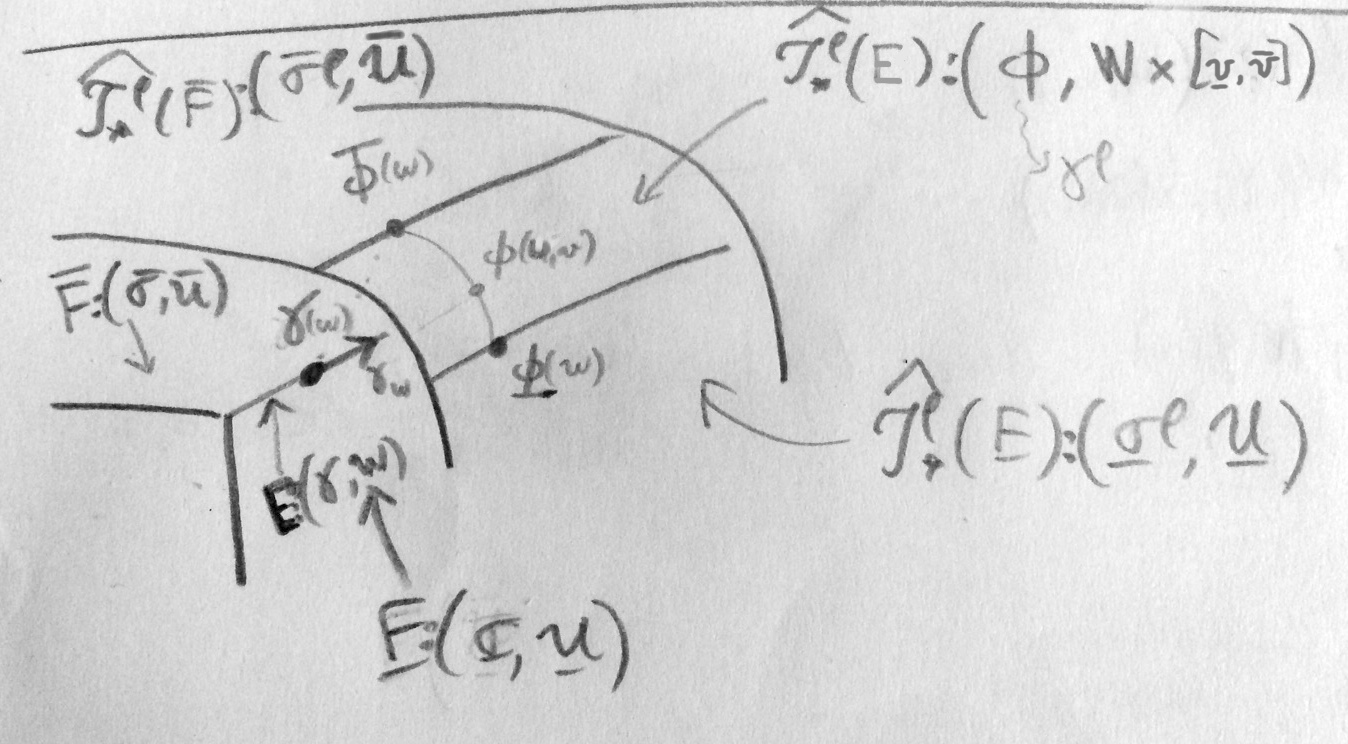
\includegraphics[width=10cm]{EdS_arete.JPG}
%    \caption{Paramétrisation de $\properEoS{\brepedge}{\rho}$}
%    \label{fig:EdS_edge}
%\end{figure}
%
%On pose $\rho = \nu \tau$.\par
%
%\newcommand{\eosR}{\lo{\vit{\eos}}}
%\newcommand{\eosL}{\hi{\vit{\eos}}}
%
%\newcommand{\psiR}{\lo{\vit{\psi}}}
%\newcommand{\psiL}{\hi{\vit{\psi}}}
%
%\newcommand{\rrwbw}{R}
%
%Soient $\brepedge$ une arête vive convexe, $\bg$ une paramétrisation de son support géométrique dans $\reals^3$ et $\lo{\brepface}$ (resp. $\hi{\brepface}$) la face à gauche\footnote{relativement à l'orientation donnée par $\bg$, vu de l'extérieur de $\Omega$.} (resp. à droite) de $\brepedge$.
%On cherche à construire un carreau paramétrique $(\mathcal{U}, \eos)$ décrivant la région de l'EdS propre de $\brepedge$ (\ie $\properEoS{\brepedge}{\rho}$) \guillemets{contenue entre}\footnote{reformuler!} $\properEoS{\lo{\brepface}}{\rho}$ et $\properEoS{\hi{\brepface}}{\rho}$ (voir \autoref{fig:EdS_edge}).\par
%On note $\lo{\bs}$ (resp. $\hi{\bs}$) une paramétrisation du carreau de surface de $\lo{\brepface}$ (resp. de $\hi{\brepface}$) et $\psiR$ (resp. $\psiL$) une paramétrisation de la trace de $\Gamma$ dans l'espace paramétrique de $\lo{\brepface}$ (resp. de $\hi{\brepface}$) telle que
%\begin{equation}
%    \bg = \lo{\bs} \circ \psiR = \hi{\bs} \circ \psiL.
%\end{equation}
%Enfin, on note $\lo{\EoB{\bs}{\rho}}$ (resp. $\hi{\EoB{\bs}{\rho}}$) la paramétrisation de $\properEoS{\lo{\brepface}}{\rho}$ (resp. de $\properEoS{\hi{\brepface}}{\rho}$) obtenue comme décrit dans la \autoref{section:paramétrisation_EdS_propre_carreau}. 
%On a alors
%\begin{equation}
%    \eosR = \lo{\EoB{\bs}{\rho}} \circ \psiR \text{ et } \eosL = \hi{\EoB{\bs}{\rho}} \circ \psiL.
%\end{equation}
%
%On choisit une paramétrisation $\eos$ de la forme \eqref{eq:eos_segment_parameterisation}, \ie les courbes iso-$u$ sont des arcs de cercles caractéristiques dont les extrémités $\eosR$ et $\eosL$ sont respectivement atteintes en $v = \lo{v}$ et $v = \hi{v}$. 
%Le domaine paramétrique est donc le rectangle $\mathcal{U} = \mathcal{W} \times \left[ \lo{v}, \hi{v} \right]$ où $\mathcal{W}$ désigne le domaine paramétrique (segment de $\reals$) de $\bg$.
%
%\par\bigskip
%
%On propose ici une méthode pour construire une telle paramétrisation. 
%\par
%[Rappeler que les courbes d'intersection sont définies de façon procédurale \ldots]
%\par
%La méthode proposée nécessite de connaître $\bg$, $\bgw$, $\eosR$ et $\eosL$ mais ne nécessite pas explicitement la donnée de $\rho$ et $\rho_w$




\subsubsection{Discrétisation de la pseudo-EdS d'un sommet \brep\ convexe}
\begin{enumerate}
	\item polygone sphérique découpé en quadrilatères (\cf \autoref{section:quadrangulation_polygone_spherique})
	\begin{itemize}
		\item construction d'un carreau bilinéaire (échantillonnage aux n\oe uds de la grille CGL)
		\item projection sur la sphère
		\item[$-$] spectre de Chebyshev plus étalé (degré plus élevé pour une précision donnée)
	\end{itemize}
	\item ajustement de carreau sphérique à un nuage de points
	\begin{itemize}
		\item échantillonnage aux n\oe uds de la grille CGL du carreau obtenu par la méthode décrite dans la \autoref{section:ajustement_carreau_spherique}
		\item[$+$] spectre de Chebyshev plus compact
	\end{itemize}
\end{enumerate}




\section{Amélioration de la stabilité numérique}
\subsection{Réduction de l'erreur d'aliasing}
méthode proposée par \cite{rahimian2015} difficile à appliquer dans notre cas car 
\begin{enumerate}
	\item les carreaux de surface ont un bord, 
	\item l'espacement non-uniforme des marqueurs lagrangiens (images des n\oe uds CGL) impose une forte contrainte CFL sur leurs déplacements
\end{enumerate}

\subsection{Prévention des singularités géométriques}
Notre approche permet naturellement de supporter les singularités géométriques de l'interface, à condition qu'elles soient localisées à l'intersection d'au moins deux carreaux de surface (et donc sur leur bord).
En revanche, les singularités qui se forment au sein d'un même carreau provoquent de sérieux problèmes de stabilité numérique.
On distingue 2 types de singularités (\cite[p.320]{patrikalakis2009}) :
\begin{itemize}
	\item points irréguliers (auto-intersection locale) (normale et plan tangent non définis, $\determinant{\fff} = 0$) $\Rightarrow$ oscillations de Gibbs
	\item auto-intersections globales (non-injectivité de la paramétrisation) : ne pose pas de problème de stabilité numérique mais viole la définition de variété
\end{itemize}

\begin{itemize}
	\item \cite{jiao2001} (en 2D, \ie l'interface est une courbe) : 
	\item \cite{farouki1986} donne les conditions pour qu'une interface (représentée par une mosaïque de carreaux paramétriques) propagée à vitesse normale uniforme devienne localement singulière
\end{itemize}

pistes de résolution envisageables
\begin{enumerate}
	\item approximation non dégénérée \cite{farouki1986}
	\item tracé des courbes iso-courbure critique \cite[chap.8]{patrikalakis2009} pour redéfinir les carreaux de surfaces concernés
\end{enumerate}

bilan : pas de solution simple, reste un gros point faible de l'approche choisie\ldots
